%!TEX root=./robocert.tex

% Metamodel references.
\newcommand{\mnamedelement}{\metaref{NamedElement}}
\newcommand{\mrapackage}{\metaref{RAPackage}}
\newcommand{\mrcpackage}{\metaref{RCPackage}}
\newcommand{\mbasicpackage}{\metaref{BasicPackage}}
\newcommand{\msequence}{\metaref{Sequence}}
\newcommand{\msubsequence}{\metaref{Subsequence}}
\newcommand{\msequencestep}{\metaref{SequenceStep}}
\newcommand{\msequencegap}{\metaref{SequenceGap}}
\newcommand{\msequenceaction}{\metaref{SequenceAction}}
\newcommand{\marrowaction}{\metaref{ArrowAction}}
\newcommand{\mloopaction}{\metaref{LoopAction}}
\newcommand{\mfinalaction}{\metaref{FinalAction}}
\newcommand{\mgapmessageset}{\metaref{GapMessageSet}}
\newcommand{\mextensionalgapmessageset}{\metaref{ExtensionalGapMessageSet}}
\newcommand{\muniversegapmessageset}{\metaref{UniverseGapMessageSet}}
\newcommand{\mmessagespec}{\metaref{MessageSpec}}
\newcommand{\marrowmessagespec}{\metaref{ArrowMessageSpec}}
\newcommand{\mgapmessagespec}{\metaref{GapMessageSpec}}
\newcommand{\mmessagetopic}{\metaref{MessageTopic}}
\newcommand{\meventmessagetopic}{\metaref{EventMessageTopic}}
\newcommand{\moperationmessagetopic}{\metaref{OperationMessageTopic}}
\newcommand{\mcspfragment}{\metaref{CSPFragment}}
\newcommand{\mnamedassertion}{\metaref{NamedAssertion}}
\newcommand{\massertion}{\metaref{Assertion}}
\newcommand{\msequenceassertion}{\metaref{SequenceAssertion}}
\newcommand{\msequenceassertiontype}{\metaref{SequenceAssertionType}}
\newcommand{\mcspmodel}{\metaref{CSPModel}}
\newcommand{\mworld}{\metaref{World}}
\newcommand{\mactor}{\metaref{Actor}}
\newcommand{\mtargetactor}{\metaref{TargetActor}}
\newcommand{\mtarget}{\metaref{Target}}
\newcommand{\mrcmodule}{\metaref{RCModule}}
\newcommand{\mrcmoduletarget}{\metaref{RCModuleTarget}}
\newcommand{\moverridetarget}{\metaref{OverrideTarget}}

This section discusses the abstract syntax (metamodel) of \langname.

\todo{Once I have a machine on which Sirius works properly, the diagrams should
be replaced with PDFs.}

\section{Packages}\label{sec:metamodel-top}

\begin{figure}
	\centering
	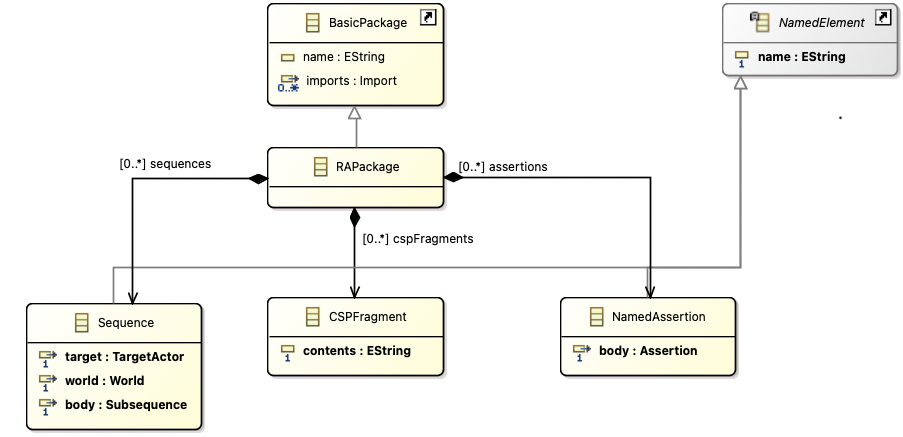
\includegraphics[width=.8\textwidth]{diagrams/top.png}
	\caption{The root of the \langname{} metamodel.}
	\label{fig:metamodel-top}
\end{figure}

\Cref{fig:metamodel-top} is the top-level metamodel diagram for \langname.

Each \langname{} script contains an \mrapackage,\footnote{\mrapackage{} stands
for `RoboStar Assertions package'; we use this name because \mrcpackage{} is
already used for RoboChart packages.}
which is a type of RoboStar \mbasicpackage.
Each \mrapackage{} can contain zero or more of each of these types of content:

\begin{itemize}
\item
	\msequence{}
	(\cref{sec:metamodel-sequences}):
	a sequence diagram;
\item
	\mcspfragment:
	a CSP fragment, currently not bound to a particular process
	\todo{this will change};
\item
	\mnamedassertion{}
	(\cref{sec:metamodel-assertions}):
	a named assertion, currently over sequence diagrams only
	\todo{more types of assertion will appear};
\end{itemize}

\todo{Elements might need to inherit from a common class and be stored in
the same list at some point.}


\section{Sequences}\label{sec:metamodel-sequences}

\begin{figure}
	\centering
	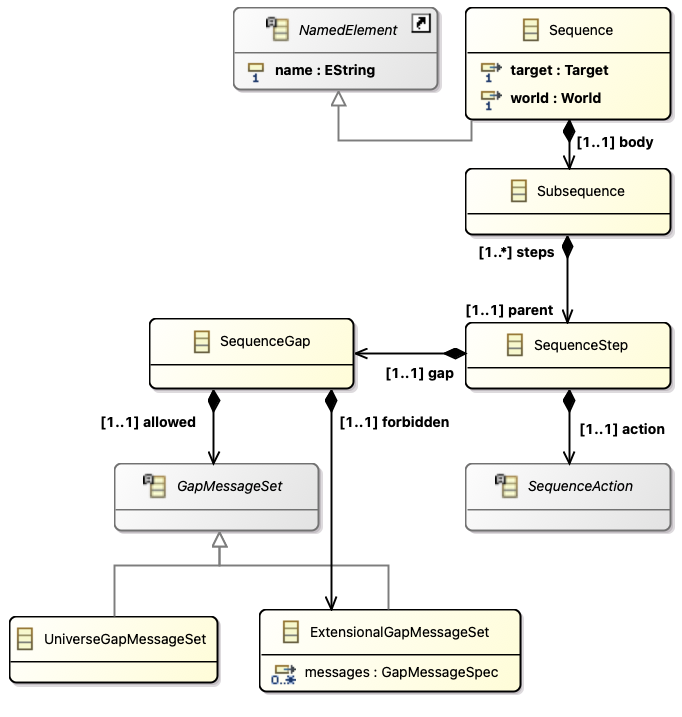
\includegraphics[width=\textwidth]{diagrams/sequences.png}
	\caption{The part of the \langname{} metamodel dealing with sequences.}
	\label{fig:metamodel-sequences}
\end{figure}

\Cref{fig:metamodel-sequences} depicts the part of the metamodel concerning
sequence diagrams.

A \msequence{} represents a single sequence diagram.  It is a \mnamedelement{}
that contains:

\begin{itemize}
\item
	a \msubsequence{} (\cref{ssec:metamodel-sequences-subsequences})
	containing the body of the diagram;
\item
	two \mactor s (\cref{sec:metamodel-actors}):
	a \mtargetactor{} (\cref{ssec:metamodel-actors-target})
	and a \mworld{} (\cref{ssec:metamodel-actors-world}).
\end{itemize}

\subsection{Subsequences}\label{ssec:metamodel-sequences-subsequences}

A \msubsequence{} is a sequential composition of one or more \msequencestep s
(\cref{ssec:metamodel-sequences-steps}).
All \msequence s contain at least one \msubsequence{} at the top level, but
may contain multiple nested \msubsequence s introduced by constructs such as
\mloopaction s.

\subsection{Steps}\label{ssec:metamodel-sequences-steps}

A \msequencestep{} is a single step in a \msubsequence.  It consists of a
\msequencegap{} (\cref{ssec:metamodel-sequences-gaps}) and a
\msequenceaction{} (\cref{sec:metamodel-sequences-actions}).

\subsection{Gaps}\label{ssec:metamodel-sequences-gaps}

A \msequencegap{} represents a condition on any communication\footnote{In PSCs,
this would correspond to \emph{intraMSG}s.} that can happen
\emph{before} a \msequenceaction.  
It contains two \mgapmessageset s: one specifying the messages
\emph{allowed} to pass inside the gap, and another specifying the messages
\emph{forbidden} to pass.\footnote{The \emph{forbidden} set is always an
\mextensionalgapmessageset, as any gap with a universal
\emph{forbidden} set would always be equivalent to one with an empty
\emph{allowed} set.
}

\paragraph{Gap message sets}

A \mgapmessageset{} is an expression of the set of messages allowed or forbidden
inside a \msequencegap.  There are two types of \mgapmessageset:

\begin{itemize}
\item
	a \muniversegapmessageset{} represents the universal set containing 
	all possible messages, and
	captures a lack of specific restriction on
	the \emph{allowed} set of a \msequencegap;
\item	
	an \mextensionalgapmessageset{} is a set (expressed as an unordered list) of
	zero or more \mgapmessagespec s, themselves
	a type of \mmessagespec{} (\cref{sec:metamodel-messages}).
\end{itemize}

There is not yet any meaningful extra data stored in
\mgapmessagespec s that is not present in \mmessagespec s, but this is subject
to change.


\subsection{Actions}\label{sec:metamodel-sequences-actions}

A \msequenceaction{} is an explicit communication or control flow construct in a
\msubsequence.  There are currently three types of action: arrow, loop, and
final actions.

\paragraph{Arrow actions}

An \marrowaction\footnote{The name signifies both that the actions resemble
PSC \emph{arrowMSG} specifications, and also that they correspond to arrows in
the graphical syntax.} specifies one communication between \mactor s which is on
the sequence specified by the diagram.  Each \marrowaction{} wraps one
\marrowmessagespec{} (\cref{sec:metamodel-messages})
containing the specification proper.
\todo{Eventually these will bind arguments.}

\paragraph{Loop actions}

A \mloopaction{} is a \emph{named} infinite loop.  \todo{Breaking and perhaps
other forms of loop are forthcoming.}  Each \mloopaction{} contains one
\msubsequence{} of steps to repeat indefinitely.
\todo{If \mloopaction s could contain zero \msubsequence s, or \msubsequence s
could contain zero \msequencestep s, they could
explicitly capture deadlock, but currently so does \mfinalaction.}

\paragraph{Final actions}

A \mfinalaction{} represents the end of a sequence diagram, corresponding
to a point in time where the sequence target has either terminated or stopped
responding.  It primarily serves to allow a final \msequencegap{} to specify
any permitted communications after the behaviour explicitly specified by the
diagram has occurred.
\todo{Is the termination behaviour correct here?  Are there any useful
parallels between this and a hypothetical empty-bodied loop action?}


\section{Message specifications}\label{sec:metamodel-messages}

\begin{figure}
	\centering
	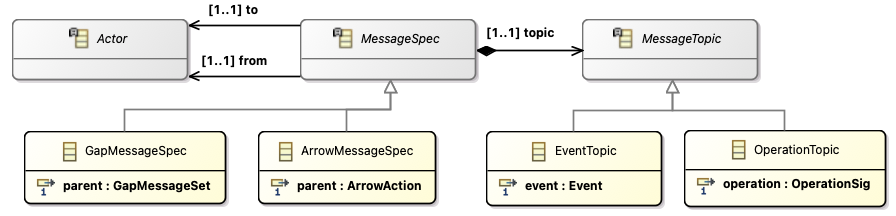
\includegraphics[width=.8\textwidth]{diagrams/messages.png}
	\caption{The part of the \langname{} metamodel dealing with messages.}
	\label{fig:metamodel-messages}
\end{figure}

\Cref{fig:metamodel-messages} depicts the part of the metamodel concerning
message specifications (`specs').

A \mmessagespec{} is a specification on the types of communication that can
happen during a gap (a \mgapmessagespec) or arrow (an \marrowmessagespec).\footnote{
This class distinction resembles that in PSCs betweeen intraMSGs and arrowMSGs,
respectively.}  Each \mmessagespec{} contains:

\begin{itemize}
\item
	references to two \mactor s, representing the \emph{to} and \emph{from}
	edges of the communication;
\item
	the \mmessagetopic{} (\cref{ssec:metamodel-messages-topics}) specifying
	the type of communication that the spec is capturing.
\end{itemize}

\subsection{Topics}\label{ssec:metamodel-messages-topics}

A \mmessagetopic{} identifies the specific type of communication in a
\mmessagespec{}.  There are currently two types of topic, corresponding to
RoboChart operations (\moperationmessagetopic) and events (\meventmessagetopic).
Each contains a reference to the signature of the respective construct.
Parameterised operations and events are not yet supported \todo{this will
change soon}.


\section{Actors}\label{sec:metamodel-actors}

\begin{figure}
	\centering
	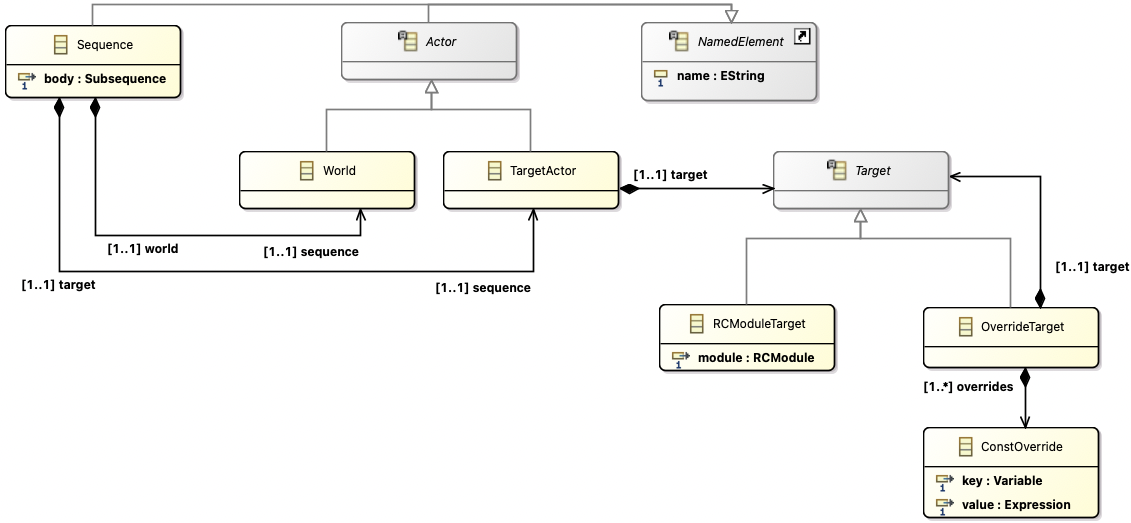
\includegraphics[width=\textwidth]{diagrams/actors.png}
	\caption{The part of the \langname{} metamodel dealing with actors.}
	\label{fig:metamodel-actors}
\end{figure}

\Cref{fig:metamodel-actors} depicts the part of the metamodel concerning
actors.

An \mactor{} is a named participant in a sequence.  The names can be used to
specify the direction of travel in \mmessagespec{}s.
As mentioned in
\cref{sec:metamodel-sequences}, there are always two actors
attached to a sequence: a \mtargetactor{} (\cref{ssec:metamodel-actors-target})
and a \mworld{} (\cref{ssec:metamodel-actors-world}).

\subsection{Targets and target actors}\label{ssec:metamodel-actors-target}

A \mtarget{} is an \emph{anonymous} specification of the part of a robotic
system that serves as the focus for a particular sequence diagram.  There are
presently two types of target, with more to appear later:

\begin{itemize}
\item
	a \mrcmoduletarget{} references a \mrcmodule;
\item
	an \moverridetarget{} wraps another \mtarget, overriding constant
	definitions.
\end{itemize}

A \mtargetactor{} wraps a \mtarget{} with a name, making it suitable as an
\mactor.  The separation between \mtarget{} and \mtargetactor{} allows for
patterns like \moverridetarget{} to exist without introducing unnecessary names.

\subsection{Worlds}\label{ssec:metamodel-actors-world}

A \mworld{} is an \mactor{} that represents the `world' outside a sequence
diagram's target.  \mworld s do not contain any data.

\section{Assertions}\label{sec:metamodel-assertions}

\begin{figure}
	\centering
	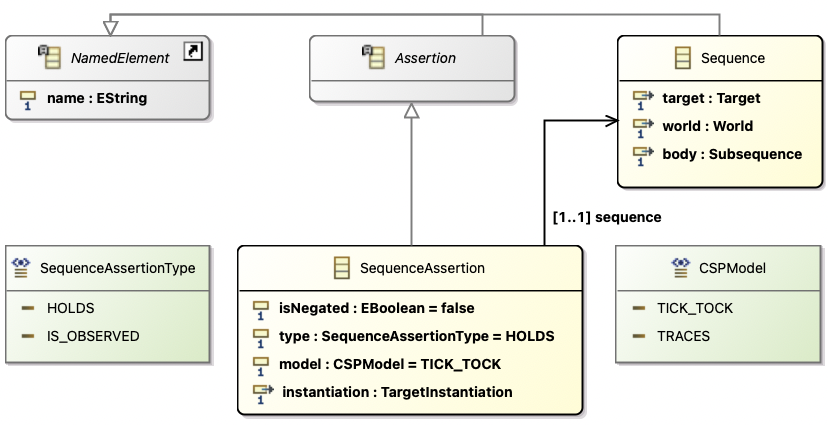
\includegraphics[width=0.7\textwidth]{diagrams/assertions.png}
	\caption{The part of the \langname{} metamodel dealing with assertions.}
	\label{fig:metamodel-assertions}
\end{figure}

\Cref{fig:metamodel-assertions} depicts the part of the metamodel concerning
assertions.

An \massertion{} is an \emph{anonymous} assertion statement.  Currently, there is
only one type of assertion: a \msequenceassertion{}.  \todo{This will change
when merging with the existing language, if not sooner.}

A \msequenceassertion{} is an assertion about a particular \msequence{} with
respect to a particular \mtarget.  By default, the \mtarget{} is that of the
\msequence{}. \todo{This isn't yet explicit in the metamodel.}  Specifying a
custom \mtarget{} as part of the assertion instead makes the assertion refer
to that target.

The specific sequence assertion type comes from the \msequenceassertiontype:
either `sequence holds on target' (refinement), or `sequence is observed on
target' (reverse refinement).  The assertion can be negated.  The choice of
\mcspmodel{} affects how the assertion is checked with CSP tools such as FDR
\todo{the models are incorrect in respect to timed assertions; I haven't yet
decided the best approach to allow the appropriate models in both timed and
untimed modes.  Currently, everything is untimed, and this too will change.}

A \mnamedassertion{} binds an \massertion{} to a name.
